\documentclass{beamer}
 \setbeamercovered{transparent}

% Used Packages
\usepackage[T1]{fontenc}
\usepackage[utf8]{inputenc}
\usepackage{graphicx}
\usepackage{listings}
\usepackage{verbatim}
\usepackage{textcomp}

% The THEME
\usetheme{Madrid}
\setbeamertemplate{navigation symbols}{}

% Title Page
\title{Distributed GPGPU Computing}
\author{Martin Stumpf}
\institute{Ste||ar Group, Louisiana State University}
\date{\today}

% Title page before every section
\AtBeginSection[]
{
   \begin{frame}
       \frametitle{Outline}
       \tableofcontents[currentsection]
   \end{frame}
}

%%%% BEGIN OF THE ACTUAL DOCUMENT %%%%
\begin{document}

\frame{\titlepage}
\frame{\frametitle{Table of Contents}\tableofcontents}

\section{GPGPU - Overview}


\subsection{GPGPU}
\begin{comment}
    Say:
        - Elements: ALU (Arithmetic logic unit), CU (controll unit),
                    Cache (L1-L3)
        - First thing to realize: More cores.
            but: every core is slower, usually ~ 1 GHz.
            also: cores are not as optimized as CPU cores
        - Next: not every core has a CU!
            this is important, one needs to take that into consideration if programming gpus.
          what does that mean?
        - GPU cores run in LOCKSTEP.
            - all of them run the same instruction at the same time.
            - can't run highly conditional code! (efficiently)
            - why use GPU's then?
\end{comment}

\begin{frame}
    \frametitle{CPU vs GPU}
    "<IMAGE GPU vs CPU>"
\end{frame}

\begin{frame}
    \frametitle{Why GPGPU?}

    The \alert{theoretical} calculation power of a GPU is much higher
    than a CPU.

    \begin{example}
        CPU (Intel Xeon E5-2670 v3):
        \begin{itemize}
            \item 12 Cores, 2.3 GHz, 32 FLOPS/cycle
            \begin{itemize}
                \item \alert{884 GFLOPS}
            \end{itemize}
            \item Prize: $\sim$ \alert{1500} \$
        \end{itemize}
        GPU (NVidia Tesla K40):
        \begin{itemize}
            \item 2880 Cores, 745 MHz, 2 FLOPS/cycle
            \begin{itemize}
                \item \alert{4291 GFLOPS}
            \end{itemize}
            \item Prize: $\sim$ \alert{4000} \$
        \end{itemize}
    \end{example}
    ~\\
    So, what computational tasks are actually suitable for GPGPU?
\end{frame}

\begin{frame}
    \frametitle{Problems suitable for GPGPU}
    Every problem that fits the \alert{SPMD} programming scheme, can benefit greatly
    from GPGPU.
    
    ~\\ 
    Examples:
    \begin{itemize}
        \item Fluid Simulations
        \item Mathematical Vector Operations
        \item Image Processing
        \item Stencil Based Simulations 
    \end{itemize}
    
    ~\\
    SPMD based Programming Languages:
    \begin{itemize}
        \item CUDA (NVidia)
        \item OpenCL (Platform independent)
    \end{itemize}
\end{frame}

\subsection{OpenCL}
\begin{frame}
    \frametitle{OpenCL}
    "<Image OpenCL host-device(kernel+buffer)>" 
\end{frame}
\begin{frame}
    \frametitle{OpenCL}
    \begin{itemize}
        \item An OpenCL device is split in two components:
        \begin{itemize}
            \item The \alert{Buffer}: Represents memory on the device
            \item The \alert{Kernel}: A C-style function that modifies one or multiple
                                      elements of a buffer
        \end{itemize}
        \item Kernel source code stays plain text and gets compiled at \alert{runtime}
        \begin{itemize}
            \item[$\implies$] OpenCL programs are device independent
        \end{itemize}
        \item Kernel executions on the device run asynchronous to the host program
    \end{itemize}
\end{frame}

\section{The MPI way}
\begin{comment}
    Say:
        - MPI and OpenCL are two independent libraries
        - connection between data exchange and calculation has to be done
          manually
        - whole cluster in lockstep
            - meaning: calculate, exchange, calculate, exchange
            - of course, you can do overlaping exchange and calculation,
              but that needs to be done manually
            - to use opencl + mpi one needs to have a lot of background knowledge
              about distributed computing
\end{comment}

\begin{frame}
    \frametitle{Distributed OpenCL with MPI}
    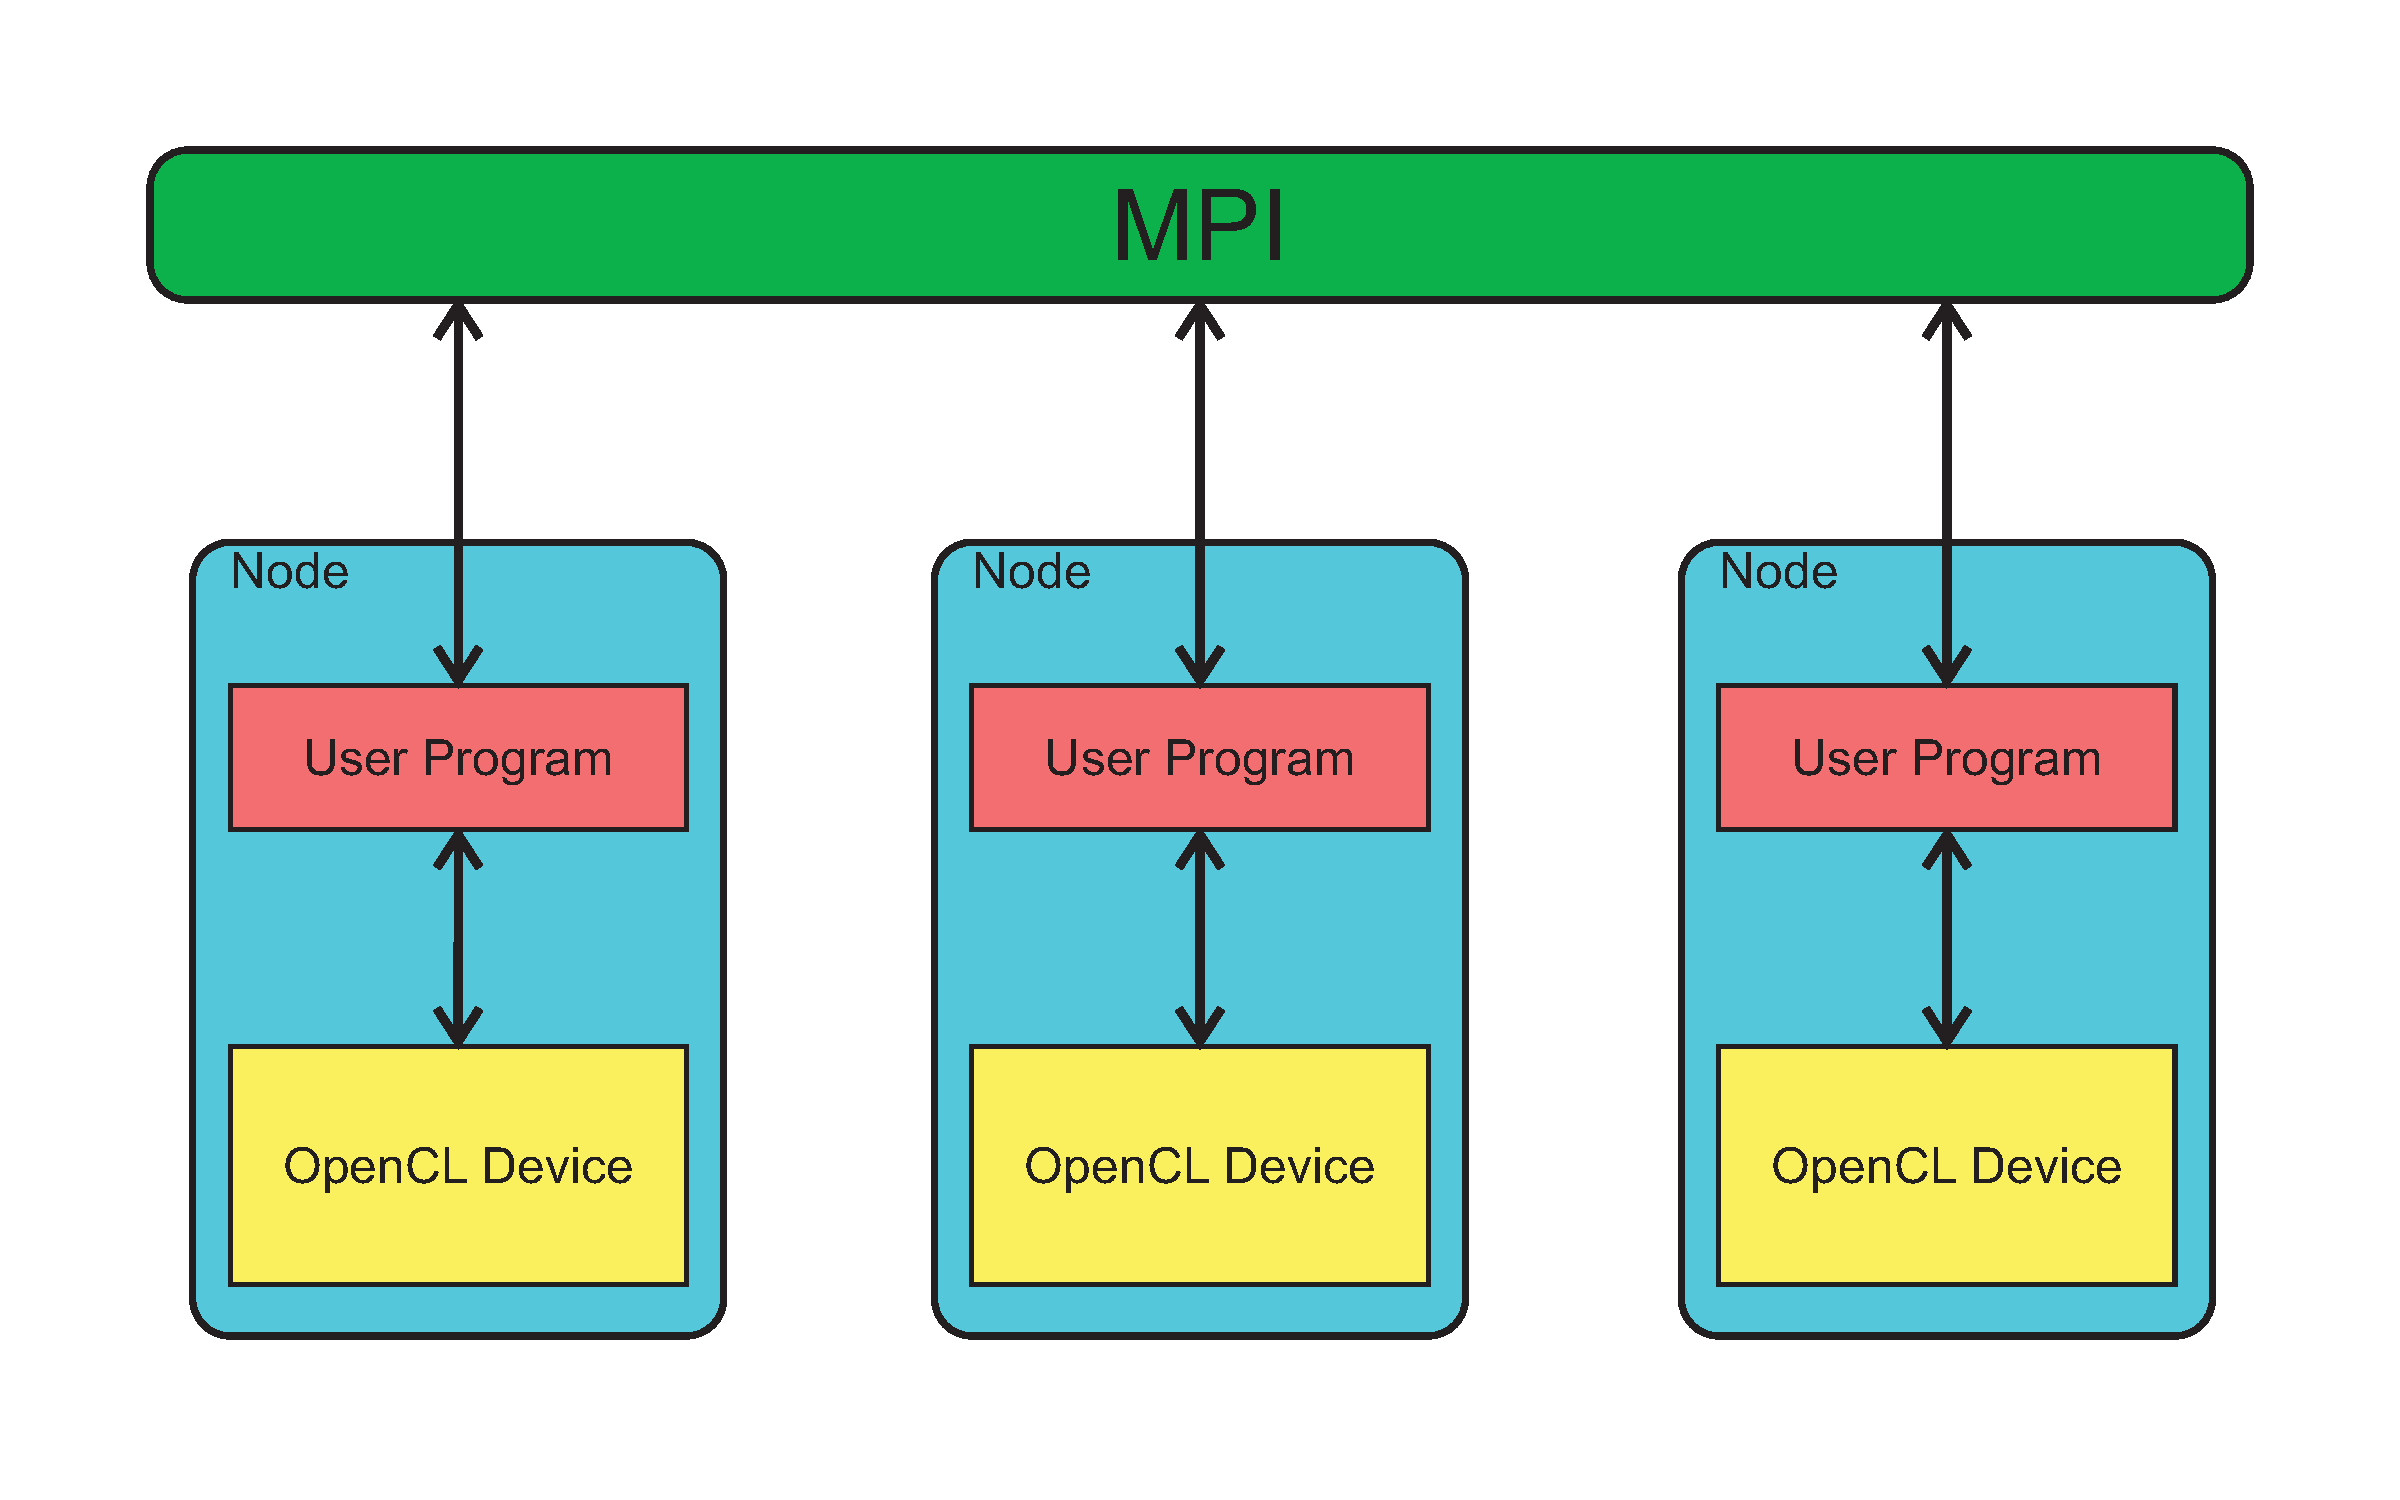
\includegraphics[width=\textwidth]{../2014-09-25_gputalk/mpi_opencl.pdf}
\end{frame}

\begin{frame}
    \frametitle{Distributed OpenCL with MPI}
    Disadvantages:
    \begin{itemize}
        \item MPI and OpenCL are independent from each other
        \begin{itemize}
            \item[$\implies$] Connection between computation and data exchange
                              has to be implemented manually
        \end{itemize}
        \item Every OpenCL device can only be accessed within its own node
        \item If no further methodes are used, the whole cluster will run in lockstep
    \end{itemize}
\end{frame}


\section{The HPX way}

\subsection{Advantages}
\begin{frame}
    \frametitle{HPX}
    What is HPX?
    \begin{itemize}
        \item A scaling C++ runtime system for parallel and distributed applications
        \item Based on the ParalleX model
    \end{itemize}
    ~\\
    Advantages for distributed OpenCL:
    \begin{itemize}
        \item Global Namespace
        \item Cluster as "one large machine" (MPI: every Node is autonomous)
        \item Data dependencies (futures) (MPI: Send-Wait)
    \end{itemize}
\end{frame}

\begin{comment}
    Say:
        Difference to MPI?
            - only one user program
            - every opencl device is now global and not just limited to the current node
            - user program can directly use remote devices
\end{comment}

\begin{frame}
    \frametitle{Distributed OpenCL with HPX}
    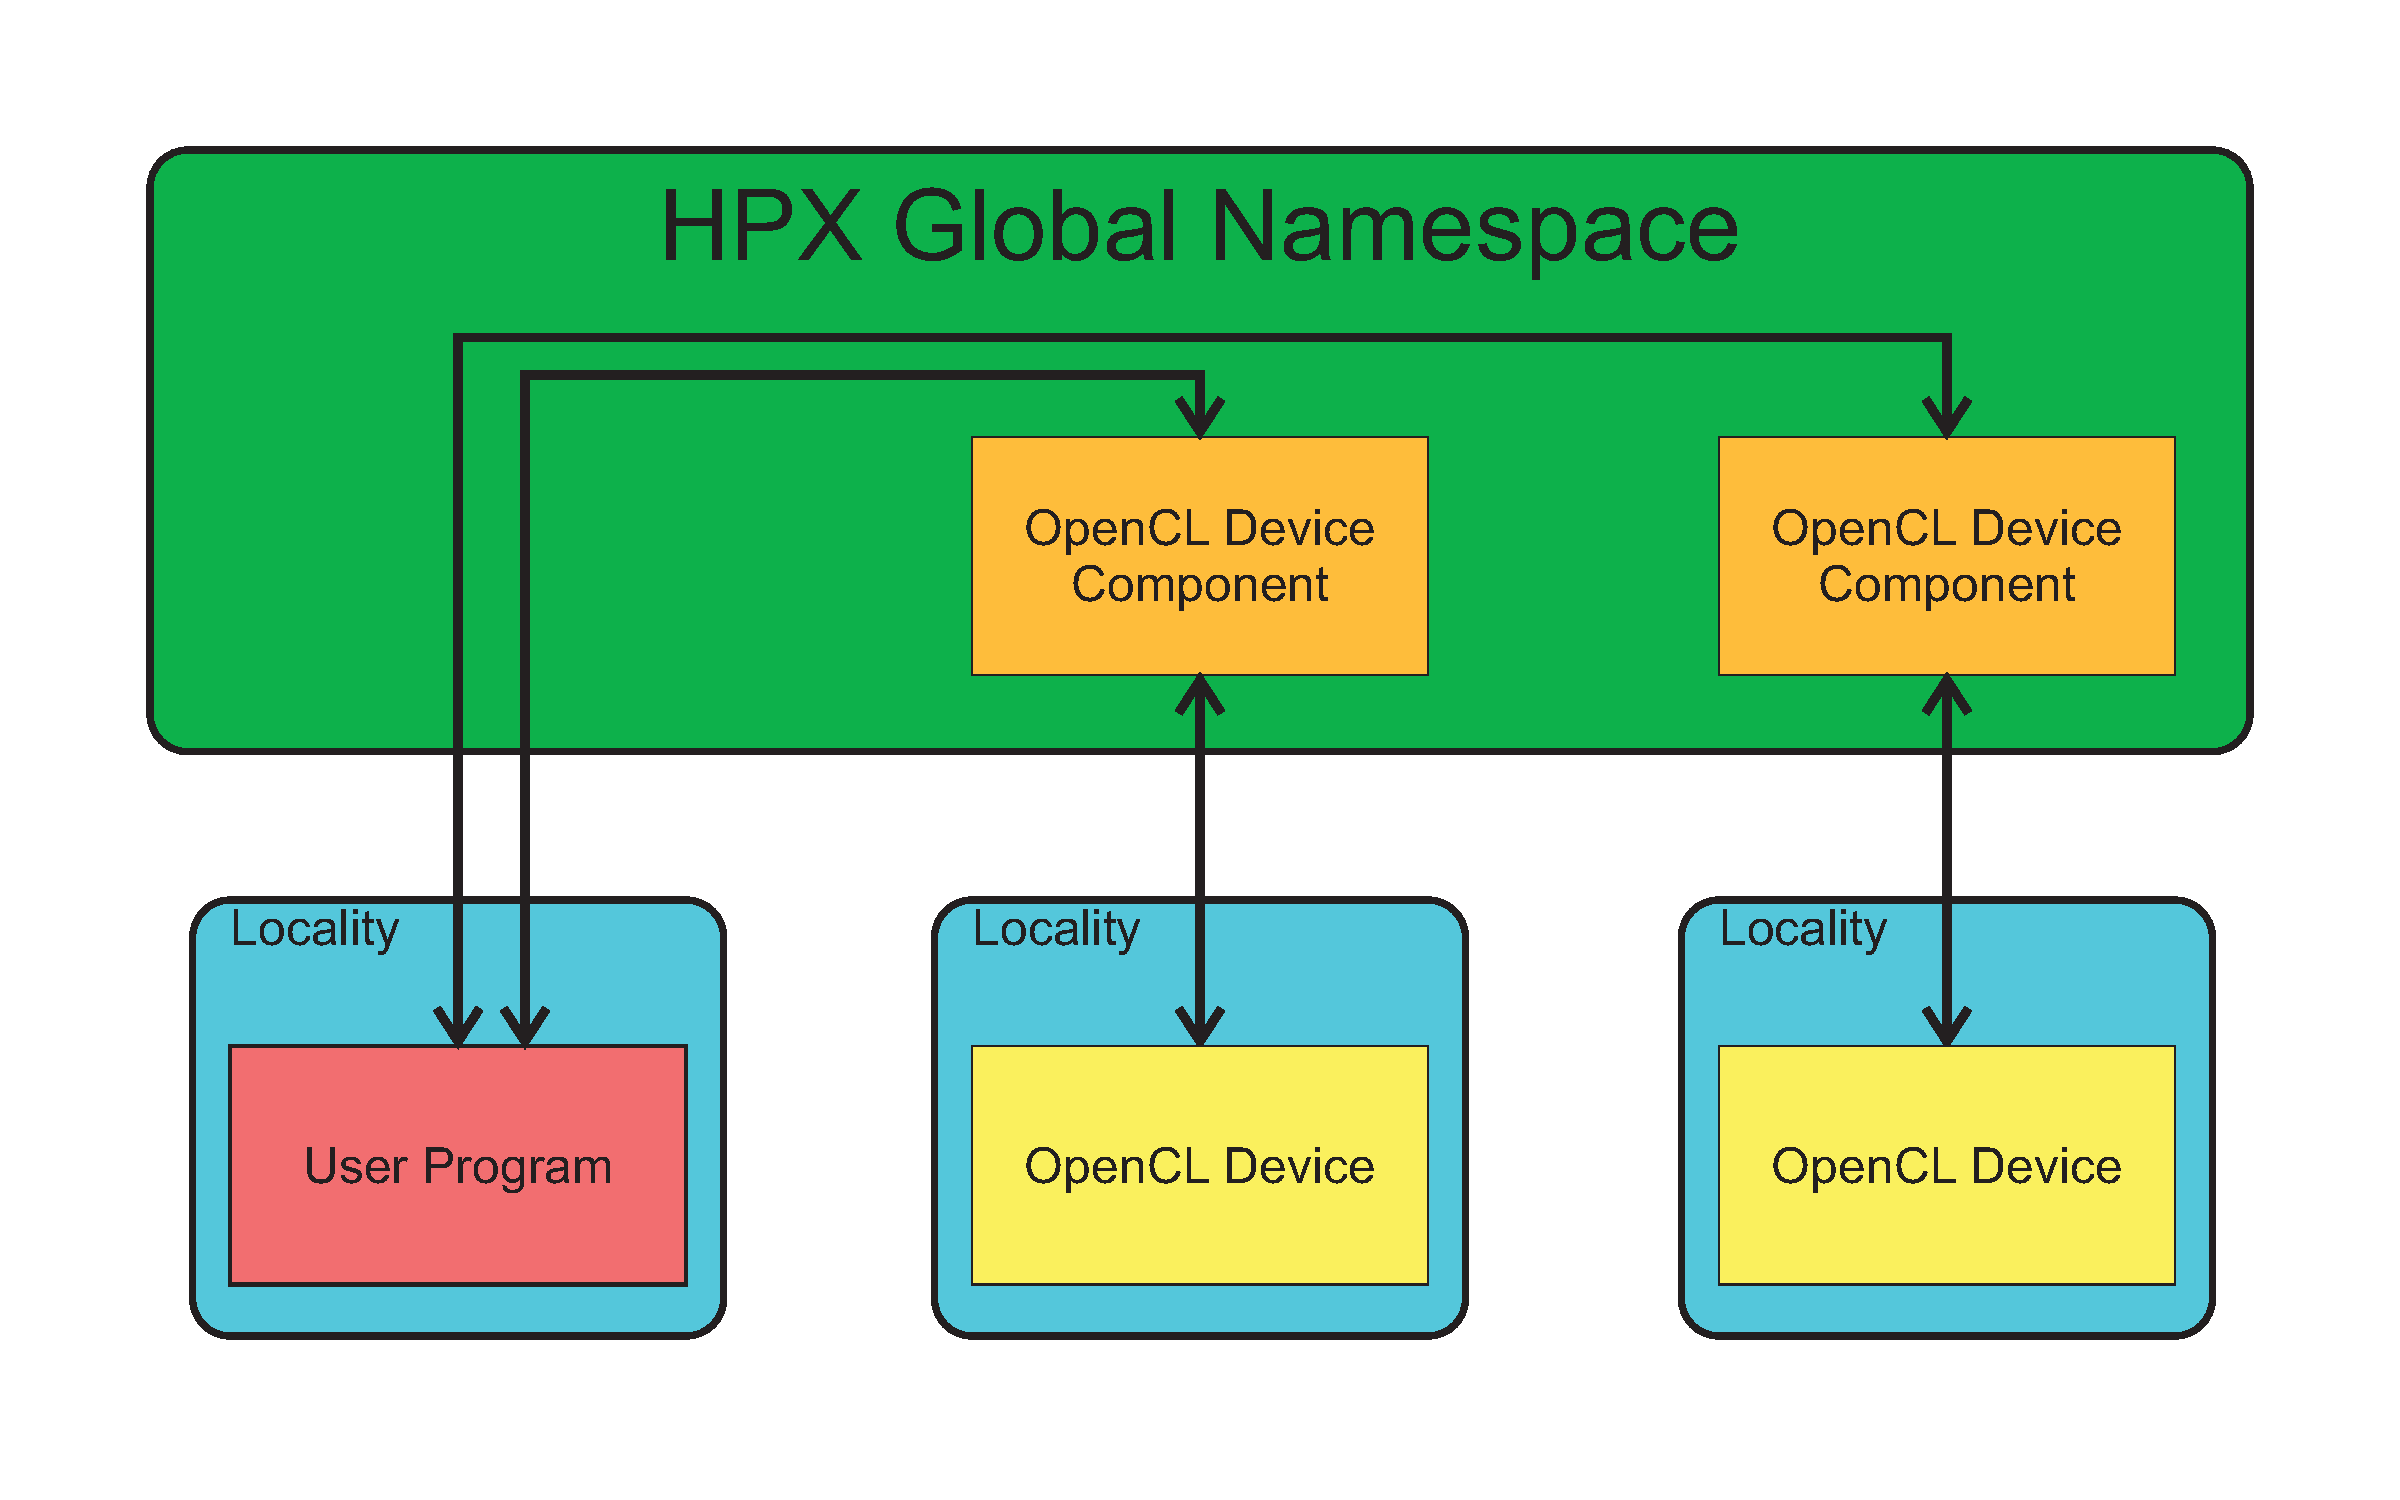
\includegraphics[width=\textwidth]{../2014-09-25_gputalk/hpx_opencl.pdf}
\end{frame}

\begin{frame}
    \frametitle{Distributed OpenCL with MPI}
    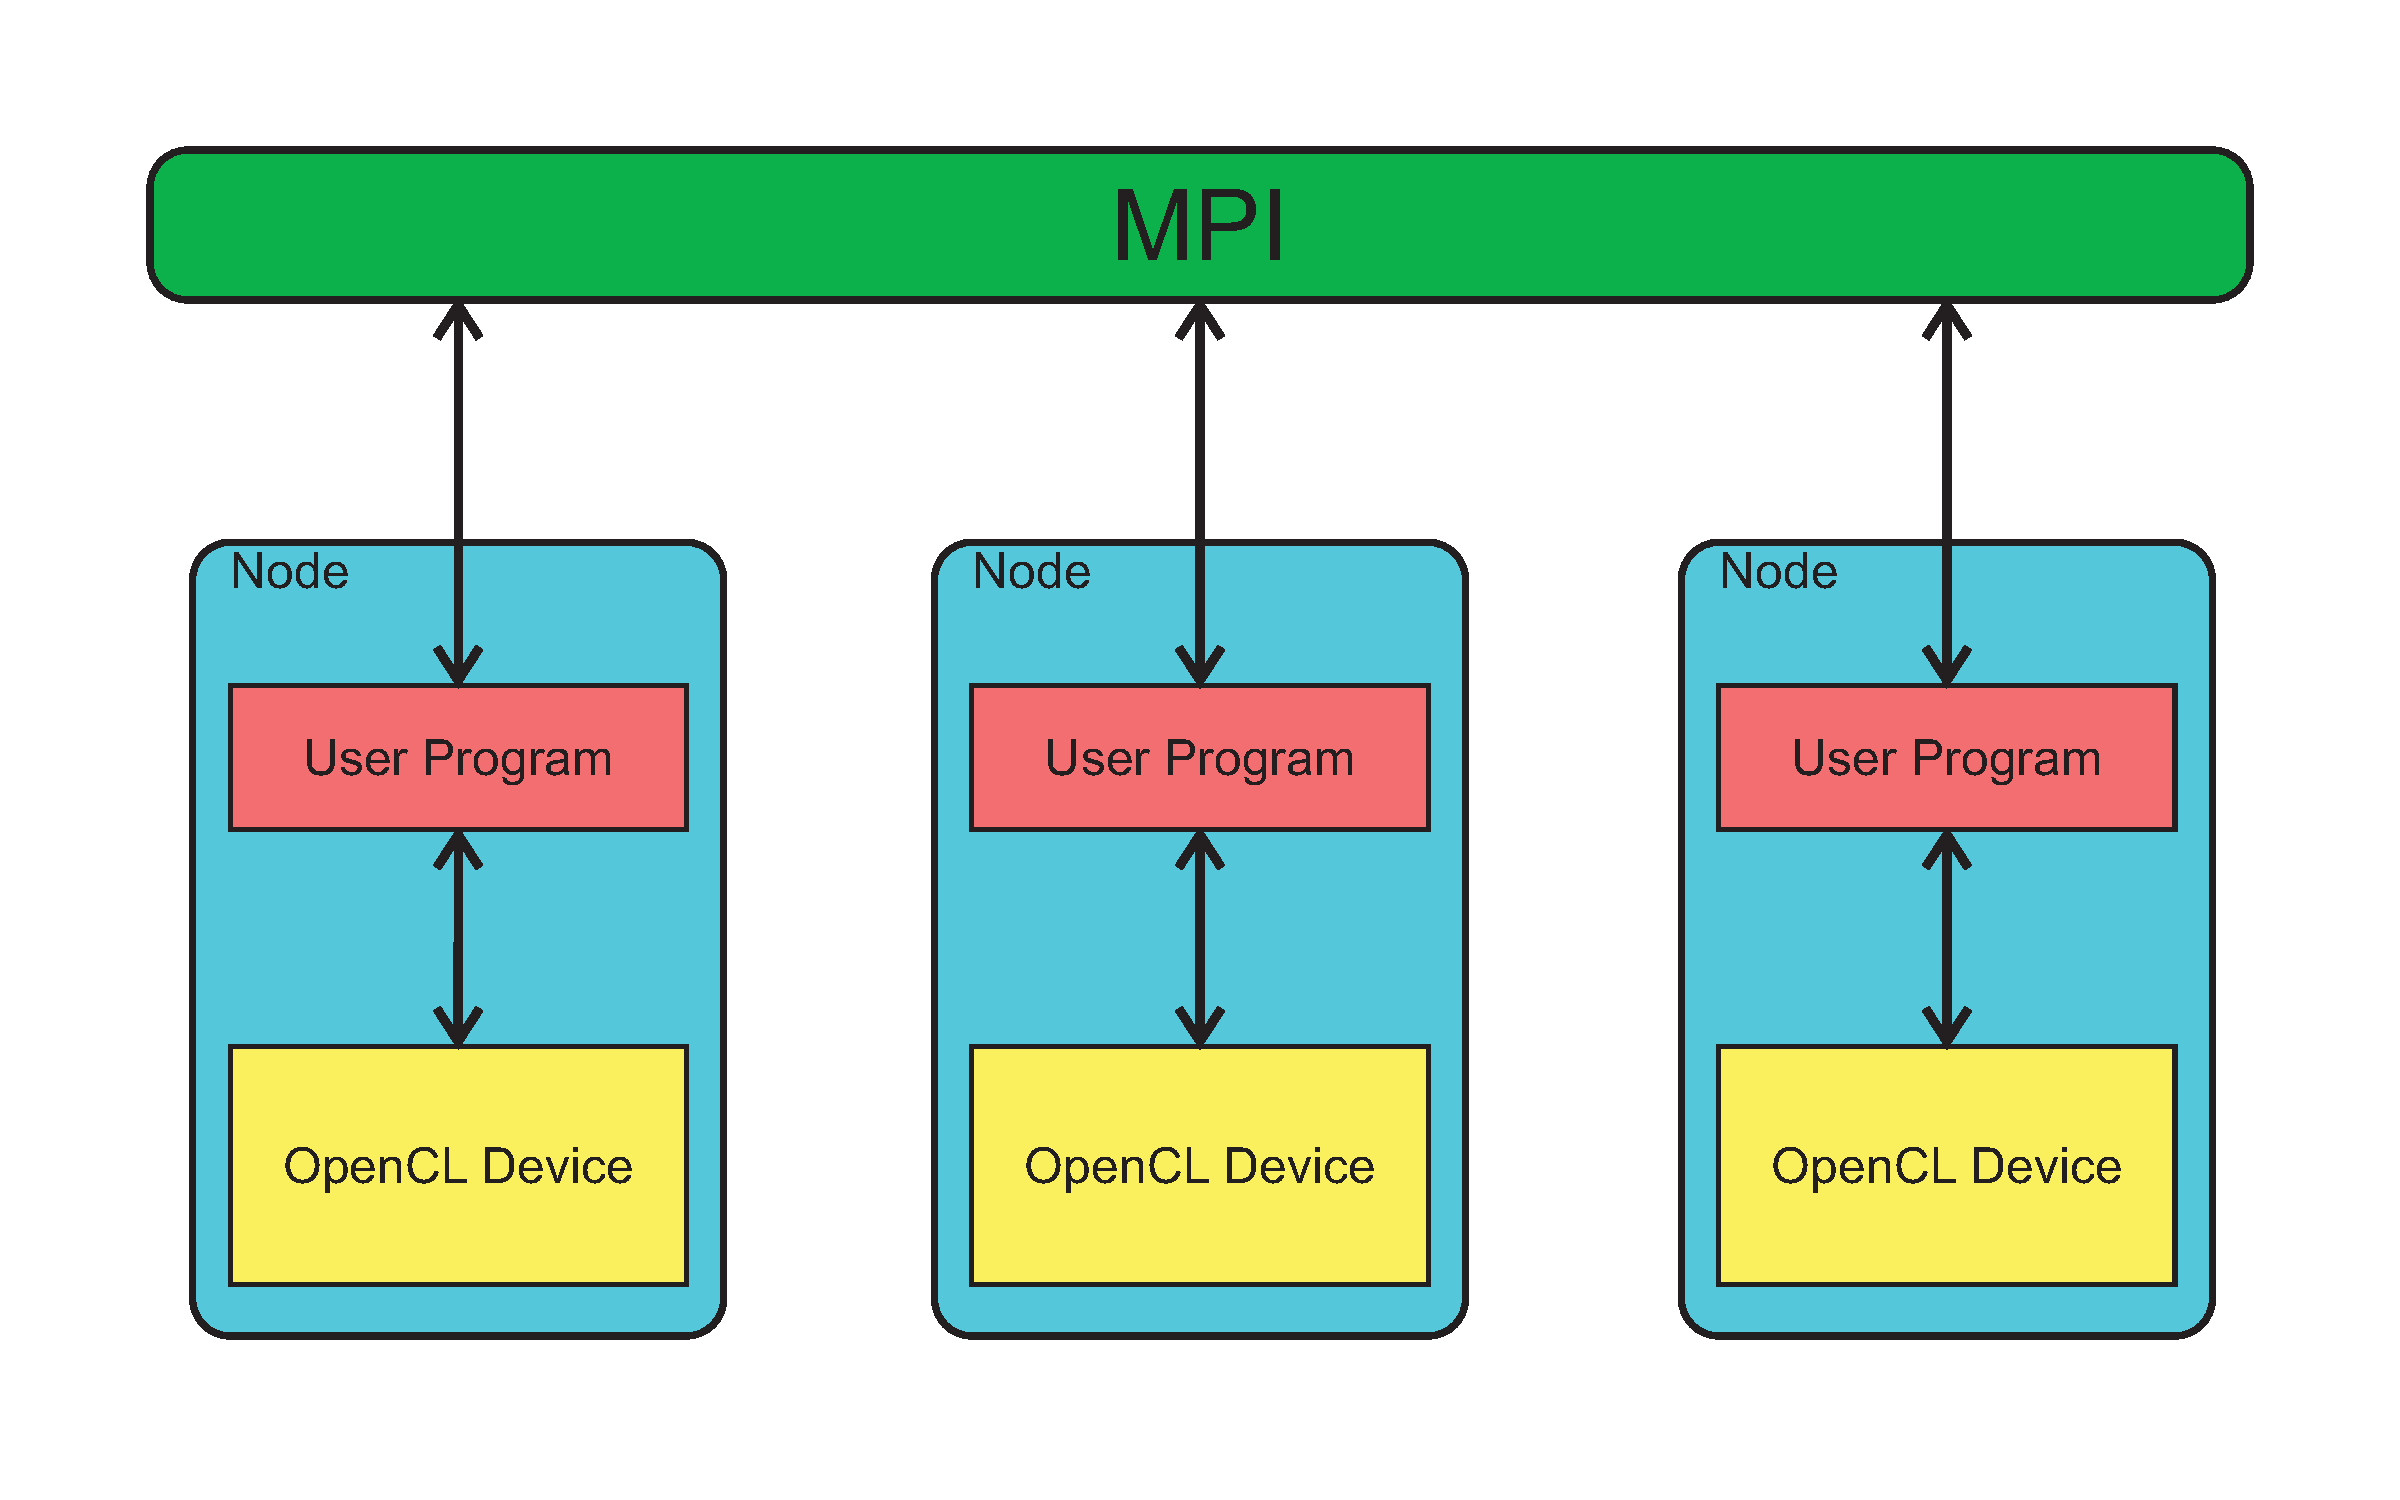
\includegraphics[width=\textwidth]{../2014-09-25_gputalk/mpi_opencl.pdf}
\end{frame}



\subsection{Affect on distributed GPGPU}
\begin{comment}
    this slide answers the question:
        what can we achieve with hpx now?
        data dependencies: due to extensive use of futures
        sync techniques of std opencl: events, data dependencies.
        someone who already knows opencl will adapt easily to the new system
\end{comment}
\begin{frame}
    \frametitle{Affect on distributed GPGPU programming}
    \begin{itemize}
        \item Abstracting the whole cluster as one machine
        \item Simpler, not need to think in a distributed way
        \item Data dependencies
        \begin{itemize}
            \item faster due to prevention of lockstep
            \item possible to apply standard OpenCL synchronization techniques
        \end{itemize}
        \item Seamless integration of more opencl nodes into the system
        \item Possibility to run heterogeneous nodes/devices in one system
        \item Easy to port non-distributed code to distributed opencl whilst
              maintaining descent scaling
    \end{itemize}
\end{frame}

\section{HPXCL}
\subsection{Layout}
\begin{frame}
    \frametitle{Layout}
    \begin{itemize}
        \item Is an implementation of that concept.
        \item Wraps every OpenCL datastructure in a component:
            \\~\\
            \begin{tabular}{ r || l }
                OpenCL       & HPXCL                \\
                \hline
                cl\_device   & hpx::opencl::device  \\
                cl\_program  & hpx::opencl::program \\
                cl\_kernel   & hpx::opencl::kernel  \\
                cl\_mem      & hpx::opencl::buffer  \\
                cl\_event    & hpx::opencl::event   \\
                ~            & (soon: hpx::future)  \\
            \end{tabular}
    \end{itemize}
\end{frame}


\subsection{Implementing "Hello, World!"}
\begin{frame}
    \frametitle{Hello, World! - Getting devices}
\end{frame}

\begin{frame}
    \frametitle{Hello, World! - Writing data to the device}
\end{frame}

\begin{frame}
    \frametitle{Hello, World! - Creating a kernel}
\end{frame}

\begin{frame}
    \frametitle{Hello, World! - Executing the kernel}
\end{frame}

\begin{frame}
    \frametitle{Hello, World! - Reading the result}
\end{frame}


\section{Performance and Scaling}

\subsection{The Mandelbrot Renderer} %TODO better title for this subsection
\begin{frame}
    \frametitle{bla}
    %about mandelbrot 
\end{frame}

\subsection{Results}

\begin{frame}
    \frametitle{Scaling}
\end{frame}

\begin{frame}
    \frametitle{Parallel Efficiency}
\end{frame}



\end{document}


     
- intro opencl
    - what is opencl?
        - open compute language
        - language for spmd problems
        - spmd?
#- intro gpu's
#    - what is a gpu?
#    - why are gpu's a good fit for opencl problems?
#    - lockstep - maybe
- distributed opencl - how?
    - MPI + OpenCL
        - Message System, data based
        - calculation, data exchange cycle
        - problem: implicit barrier between steps
        - problem: explicit distribution
- HPX        
        - what is HPX?
        - async RPC based
        - calculation, dependency tree
        - good fit for opencl, as opencl is in itself also dependency based
        - easy to program, use cluster as if it were a single machine
- HPXCL

- POCL?

